\documentclass[a4paper,12pt]{article}

\usepackage{a4wide}
\usepackage{amsmath}
\usepackage{amssymb}
\usepackage{amsthm}
\usepackage[czech]{babel}
\usepackage{bookmark}
\usepackage{enumerate}
\usepackage[T1]{fontenc}
\usepackage{forest}
\usepackage{hyperref}
\usepackage[utf8]{inputenc}
\usepackage{lmodern}
\usepackage{multicol}
\usepackage{tikz}

\theoremstyle{definition}
    \newtheorem{problem}{Příklad}

% \theoremstyle{remark}
%     \newtheorem*{steps}{Postup řešení}

\theoremstyle{plain}
    \newtheorem*{solution}{Řešení}
    

\DeclareRobustCommand\proves{\mathrel{|}\joinrel\mkern-.5mu\mathrel{-}}
\DeclareMathOperator{\Conseq}{Csq}
\DeclareMathOperator{\M}{M}

% hide solutions
\newif\ifhidesolutions
    \hidesolutionstrue
    % \hidesolutionsfalse

\ifhidesolutions
    \usepackage{environ}
    \NewEnviron{hide}{}
    \let\solution\hide
    \let\endsolution\endhide
\fi









\begin{document}

\section*{NAIL062 V\&P Logika: 6. cvičení}
% druhé cvičení po 4. přednášce

% 2023: 1, 2, 3a, 4, 5ab


\textbf{Témata:} 
Ještě tablo metoda: aplikace a pokročilejší problémy. Ukázka rezoluční metody.



\medskip\begin{problem}
    Aladin našel v jeskyni dvě truhly, A a B. Ví, že každá truhla obsahuje buď poklad, nebo smrtonosnou past.
    \begin{itemize}
    \item Na truhle A je nápis: {\it ``Alespoň jedna z těchto dvou truhel obsahuje poklad.''}
    \item Na truhle B je nápis: {\it ``V truhle A je smrtonosná past.''}
    \end{itemize}
    Aladin ví, že buď jsou oba nápisy pravdivé, nebo jsou oba lživé.
    \begin{enumerate}
        \item Vyjádřete Aladinovy informace jako teorii $T$ nad vhodně zvolenou množinou výrokových proměnných $\mathbb P$. (Vysvětlete význam jednotlivých výrokových proměnných v $\mathbb P$.)
        \item Pomocí tablo metody najděte všechny modely teorie $T$.
        \item Může Aladin zvolit truhlu tak, aby si byl jistý, že v ní bude poklad?
    \end{enumerate}
    \end{problem}
    
    
    \medskip\begin{problem} % a bit larger tableaux
    V prezidentských volbách kandidují pan A a pan B.
    \begin{itemize}
    \item Pan A říká: {\it ``Budu zvolen nebo pan B lže.''}
    \item Pan B říká: {\it ``Pan A nebude zvolen nebo lžu.''}
    \item Bude zvolen právě jeden z nich.
    \end{itemize}
    \begin{enumerate}
    \item Formalizujte jako teorii $T$ v jazyce $\mathbb P=\{z_a,z_b,p_a,p_b\}$, kde $z_a$ resp. $z_b$ znamená, že zvolen bude pan A resp. pan B, a $p_a$ resp. $p_b$ znamená, že A resp. B mluví pravdu.
    \item Sestrojte dokončená tabla z teorie $T$ s položkami $\mathrm{F}z_a$ resp. $\mathrm{F}z_b$ v kořeni. Jaký z těchto tabel můžeme učinit závěr? [Tabla mohou být poměrně velká.]
    \item Uveďte příklad výroku nad $\mathbb{P}$, který je v teorii $T$ nezávislý, anebo zdůvodněte, proč takový výrok neexistuje.
    \item Existuje teorie $S$ nad $\{z_a,z_b\}$ taková, že $T$ je konzervativní extenzí $S$? Uveďte příklad, nebo zdůvodněte, proč ne.
    \end{enumerate}
\end{problem}


\medskip\begin{problem}
    Uvažme nekonečnou výrokovou teorii (a) $T=\{p_{i+1} \to p_i\mid i\in \mathbb{N}\}$ (b) $T=\{p_i \to p_{i+1}\mid i\in \mathbb{N}\}$. Pomocí tablo metody najděte všechny modely $T$. Je každý model $T$ kanonickým modelem pro některou z větví tohoto tabla? (Můžete se pokusit sestrojit také \emph{systematické} tablo.)
\end{problem}


\medskip\begin{problem} 
    Navrhněte vhodná atomická tabla a ukažte, že souhlasí-li model s kořenem vašich atomických tabel, souhlasí i s některou větví:
    \begin{itemize}
        \item pro Peirceovu spojku $\downarrow$ (NOR),
        \item pro Shefferovu spojku $\uparrow$ (NAND),
        \item pro $\oplus$ (XOR),
        \item pro ternární operátor ``if p then q else r'' (IFTE).
    \end{itemize}  
    
\end{problem}


\medskip\begin{problem}
    \emph{Half-adder circuit} je logický obvod se dvěma vstupními bity (bit 1, bit 2) a dvěma výstupními bity (carry, sum) znázorněný v následujícím diagramu:
    \begin{center}
        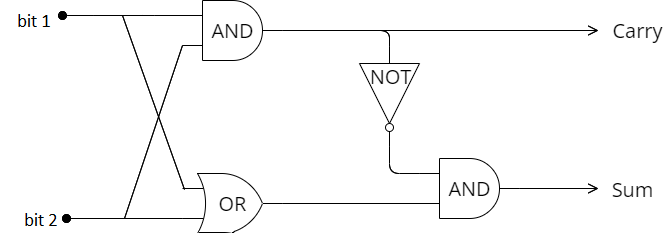
\includegraphics[width=0.5\textwidth]{files/half-adder.png}
    \end{center}
    \begin{enumerate}
            \item Formalizujte tento obvod ve výrokové logice. Konkrétně, vyjádřete jej jako výrokovou teorii $T=\{c\leftrightarrow \varphi,\ s\leftrightarrow \psi\}$ v jazyce $\mathbb P=\{b_1,b_2,c,s\}$, kde výrokové proměnné znamenají po řadě ``bit 1'', ``bit 2'', ``carry'' a ``sum'', a formule $\varphi,\psi$ neobsahují proměnné $c,s$.
            %\item Axiomatizujte teorii $T$ výrokem v CNF a také výrokem v DNF
            \item Dokažte tablo metodou, že $T\models c\to\neg s$.
            \item Dokažte totéž rezoluční metodou (připomeňte si ji).
    \end{enumerate}
\end{problem}



\medskip\begin{problem}
        Dokažte přímo (transformací tabel) větu o dedukci, tj. že pro každou teorii $T$ a výroky $\varphi$, $\psi$ platí
        $$T \proves \varphi\to\psi\text{\ \ právě když\ \ }T,\varphi\proves  \psi.$$
\end{problem}


\medskip\begin{problem}
    Celá čísla postihla záhadná nemoc šířící se (v diskrétních krocích) dle následujících pravidel (platících pro všechna čísla ve všech krocích).
    \begin{enumerate}[label=(\roman*)]\it
    \item Zdravé číslo onemocní, právě když je právě jedno číslo nemocné (v předchozím čase).
    \item Nemocné číslo se uzdraví, právě když je předchozí číslo nemocné (v předchozím čase).
    \item V čase $0$ bylo nemocné číslo $0$, ostatní čísla byla zdravá.
    \end{enumerate}
    %(Sousedními čísly čísla $i$ myslíme $i-1$ a $i+1$, předchozím číslem myslíme $i-1$.)
    \begin{enumerate}
    \item Napište teorie $T_1, T_2, T_3$ vyjadřující (po řadě) tvrzení $(i), (ii), (iii)$ nad množinou prvovýroků $\mathbb{P}=\{p_i^t \mid i\in\mathbb{Z}, t\in\mathbb{N}_0\}$, kde prvovýrok $p_i^t$ vyjadřuje, že ``{\it číslo $i$ je v čase $t$ nemocné.}''
    \item Převeďte axiomy z $T_1, T_2, T_3$ do CNF a napište teorii $S$ v množinové reprezentaci, která je nesplnitelná, právě když $T_1 \cup T_2 \cup T_3 \models \neg p_1^2$, tj.: ``{\it Číslo $1$ je zdravé v čase $2$.}'' (Stačí převést jen konkrétní axiomy z $T_1,T_2,T_3$, ze kterých plyne $\neg p_1^2$, a do $S$ uvést jen příslušné klauzule.)
    \item Rezolucí dokažte, že $S$ je nesplnitelná. Zamítnutí znázorněte rezolučním stromem.
    \end{enumerate}
\end{problem}

 


\end{document}